% !TeX spellcheck = sk_SK-Slovak
\chapter{Vstupné dáta a ich štruktúra}

\label{kap:strukSpravy} % id kapitoly pre prikaz ref

Táto kapitola sa zameriava na pochopenie vstupných dát a približnú lokalizáciu hľadaných informácii v nich.

\section{Zdroj dát}

Prepúšťacie správy a krvné výsledky ktoré náš systém spracováva sú správami pacientov ktorý boli v období od marca roku 2020 do decembra roku 2021 hospitalizovaný na klinike infektológie a geografickej medicíny univerzitnej nemocnice v Bratislave.

\section{Výzor vstupných dát}

Dáta z ktorých sa snažíme získať informácie o pacientovi softvér dostáva v tvare textu obsahujúceho prepúšťaciu správu a krvné výsledky. Väčšina textu v prepúšťacej správe nie je generovaná automaticky nemocničným informačným systémom ale je písaná lekárom čo spôsobuje, že každá správa je do určitej miery originálna.

Napriek tomu existuje základná štruktúra ktorú majú spoločnú takmer všetky prepúšťacie správy vďaka ktorej je možné túto správu rozdeliť do blokov (viď obrázok \ref{obr:sprava}) ktoré obsahujú určitý informácie. Teraz si prejdeme, čo obsahujú jednotlivé bloky a čo z nich sa mi snažíme získať.

\begin{figure}
	%vlozenie samotneho obrazku vycentrovaneho a vhodnej velkosti
	%obrazok je v subore images/cervik.png
	\centerline{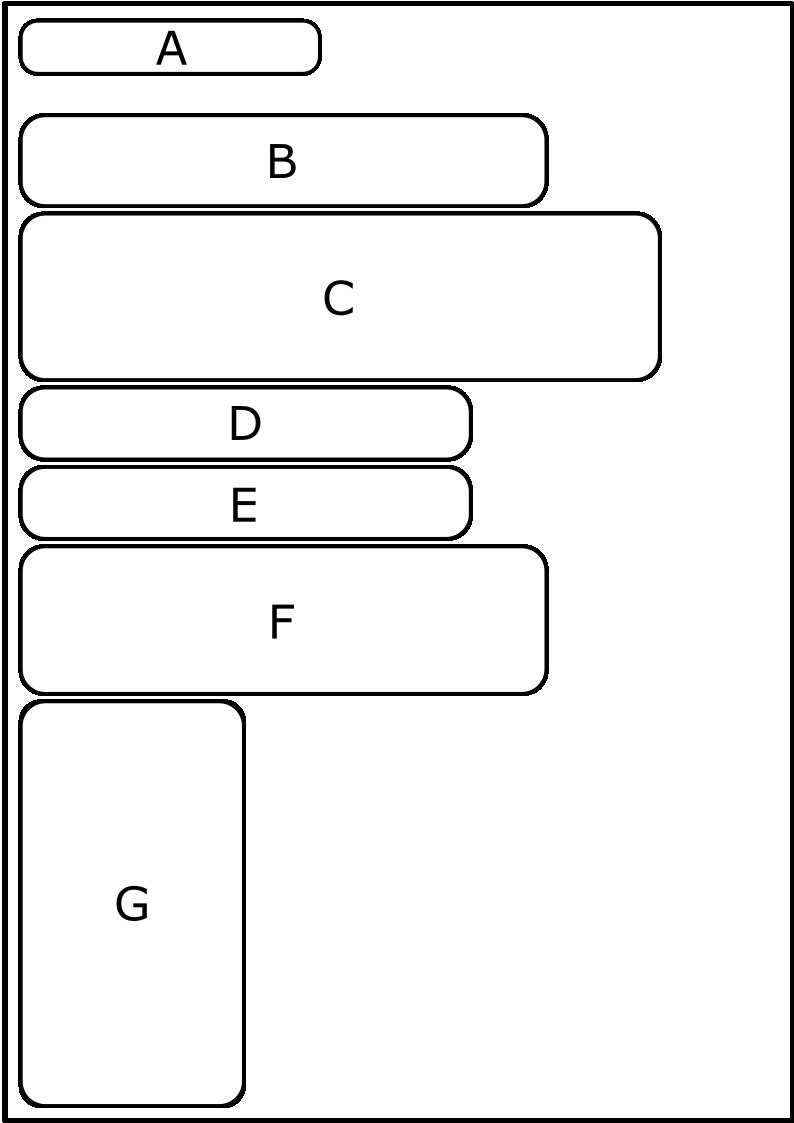
\includegraphics[width=0.4\textwidth]{images/vyzor_spravy}}
	%popis obrazku
	\caption[Rozloženie správy]{Rozdelenie správy do špecifických blokov podľa ich obsahu}
	%id obrazku, pomocou ktoreho sa budeme na obrazok odvolavat
	\label{obr:sprava}
\end{figure}

\subsection{Blok A - Osobné údaje a obdobie hospitalizácie}
\label{blokA}
Bloku A je dvojriadková hlavička v ktorej sa nachádzajú osobné údaje pacienta, čiže jeho celé meno a rodné číslo, a zároveň sa tam nachádza dátum priatia a dátum prepustenia daného pacienta. Všetky tieto informácie sa snažíme získať.

\subsection{Blok B - Anamnéza}
\label{blokB}
Tento blok obsahuje informácie o anamnéze a stave pacienta pri prijatí do nemocnice, z tohto bloku sa snažíme získavať informácie ako sú výška, váha a saturácia krvi kyslíkom pri prijatí, a informácia o dlhodobých alebo v minulosti prekonaných chorobách a problémoch ako sú cukrovka, astma, demencia, infarkt myokardu, artériová hypertenzia, fibrilácia predsiení, srdcové zlyhanie a ďalšie.

\subsection{Blok C - Vyšetrenia}
\label{blokC}
Blok C obsahuje informácie o vykonaných vyšetreniach, pre nás sú podstatné výsledky testov na protilátky proti vírusu SARS-CoV-2 typu IgG a IgM pri prijatí, prípadne výsledok testu na ochorenie CDI (Infekcia spôsobená Clostridium difficile).

Zároveň sa tu nachádzajú aj výsledky krvných testov avšak tie sa tu nemusia nachádzať úplné. Preto softvér ktorým to spracovávame ich považuje za kontrolné a samotné informácie o krvných výsledkoch sa získavajú z posledného bloku (\ref{blokG}).

\subsection{Blok D - Terapia}
\label{blokD}
V tomto bloku sú informácie o terapii odtiaľto získavame informáciu o liekoch ktoré boli pacientovi podané počas hospitalizácie a o tom či pacient potreboval aj oxygenoterapia a v prípade, že áno aj o aký typ oxygenoterapie išlo.

\subsection{Blok E - Epikríza}
\label{blokE}
Tento blok obsahuje časť správy s názvom epikríza čiže záverečná, súhrnná správa o pacientovi, priebehu jeho choroby a hospitalizácie. Jedinou získavanou informáciou je informácie o smrti pacienta. Táto časť sa však dá zároveň využiť aj na prípadnú kontrolu iných získavaných informácii keďže môže obsahovať informáciu o iných ochoreniach pacienta, jeho liečbe, prípadne o prítomnosti protilátok proti vírusu SARS-CoV-2.

\subsection{Blok F - Záver, odporúčania, špecifické nálezy}

Blok F obsahuje zvyšné časti správy ako sú záver, odporúčania a špecifické nálezy. Avšak obsah tohto bloku je výrazne nekonzistentný a jeho jednotlivé časti nemusia byť vôbec prítomné v správe. Našťastie tento blok by nemal neobsahovať žiadne konkrétne získavané informácie.

\subsection{Blok G - Krvné výsledky}
\label{blokG}
Záverečný blok už nie je priamo prepúšťacia správa ale ide o krvné výsledky pacienta ktoré narozdiel od výsledkov v bloku C (\ref{blokC}) sa tu nachádzajú úplné a zároveň vďaka tomu, že nie sú napísané vedľa seba ako v bloku C ale pod sebou (každý výsledok na samostatnom riadku) je práca s nimi výrazne jednoduchšia.

\section{Problémy pri rozdelení dát na bloky} 

Pri snahe o implementácia tohto delenia sme zistili, že aj napriek tomu, že sa pomerne veľký počet správ dal do takýchto blokov rozdeliť, tak sa objavilo niekoľko problémov či už pri samotnom delení správy ako aj pri informačnom obsahu jednotlivých častí kvôli ktorým sa ukazuje vhodnejšie takéto riešenie vôbec nepoužiť alebo použiť nejakú robustnejšiu verziu tohto delenie. Niektoré z nájdených problémov si teraz opíšeme.

\subsection{Problém nenájdených blokov}

Pri kontrole správ rozdelených do blokov sme zistili, že sa občas stávalo, že náš softvér nebol schopný nájsť niektorý z blokov, väčšinu z týchto problémov vieme rozdeliť do troch skupín: chýbajúci alebo nesprávne ohraničený blok F, blok E skrytý v bloku F, chýbajúci alebo nesprávne napísaný začiatok bloku.

Prvý problém pre nás nepredstavuje veľký problém keďže v bloku F by sa nemali nenachádzajú hľadané informácie. 

Druhý problém je o niečo horší keďže blok E je pre nás dôležitý ale tento problém bolo jednoduché opraviť tým, že ak softvér nenájde blok E pri prvotnom delení správy ešte skontroluje či sa v bloku F náhodnou nenachádza.

Tretí problém sa ukazuje ako najproblematickejší sa ukázalo ako pomerne komplikované určiť začiatok a koniec bloku ak softvér nenájde kľúčové slová ktorými sa vo väčšine prípadov jednotlivé bloky začínajú a preto sa stávalo, že softvér niektoré bloky nenašiel a lebo ich pripojil k iným blokom. Tento problém sa stal jedným z hlavných zmeny prístupu k dátam.

\subsection{Problém nesprávne umiestnených dát}

Ako ďalší veľký problém sa ukazuje to, že niektoré informácie sa nenachádzajú sa očakávanom mieste. Zväčša išlo o informácie o anamnéze pacienta a výsledkoch jeho vyšetrení ktoré sme predpokladali, že nájdeme v blokoch B respektíve C avšak časť týchto informácii sa nachádzala až v bloku F.

Tento problém samotný sa dá riešiť tým, že informácie ktoré hľadáme v blokoch B a C budeme nakoniec hľadať avšak tento problém spôsobuje, že problém ktorý máme s nájdením a správnym ohraničením bloku F sa stáva relevantným a treba ho riešiť, nanešťastie tento problém je podobný problému ohraničeniu ostatných blokov a preto je jeho riešenie pomerne komplikované.

\section{Riešenia problémov s rozdelením dát do blokov}

Skúšaním rôznych spôsobov riešenia sa ukázalo, že najvhodnejšie je neriešiť okrajové prípady súčasného rozdelenia správy ale prerobiť samotné rozdeľovanie. {Našli sme najlepšie spôsoby...}

\subsection{Homogénny text}

Jednou možnosťou je považovať celý text ako jeden homogénny text v ktorom hľadáme všetky informácie.

Tento prístup rieši všetky naše problémy avšak zbytočne hľadá niektoré informácie aj na miestach kde vieme, že sa nikdy nebudú nachádzať čo ho spomaľuje.

\subsection{Menej väčších blokov}
\label{spravaLepsie}

Tento prístup využíva rozdelenie do blokov ale namiesto pôvodných 7 blokov toto nové rozdelenie má iba 3 bloky, vďaka čomu nemusí hľadať všetky informácie v celom texte a zároveň pri správnom rozdelení vyriešime problémy ktoré sa v pôvodnom rozdelení objavili. 

Výzor nového rozdelenia môžeme vidieť na obrázku \ref{obr:sprava_uprava}. Vidíme, že jediná zmena ktorá nastala je taká, že sme bloky B až F spojili do jedného bloku s názvom B a pôvodný blok G sme premenovali na blok C. 

Toto rozdelenie rieši všetky vyššie spomenuté problémy vďaka tomu, že o bloku A vieme, že vždy bude mať tvar dvojriadkovej hlavičky s pri skúšaní sme nenašli žiadnu výnimku, podobne pôvodný blok G čiže nový blok C nie je súčasťou samotnej prepúšťacej správy ale sú to krvné výsledky pacienta ktoré sú v našom vstupe vždy až za správou a majú tvar dvojíc testovaná veličina a výsledok testu (pozitivita alebo hodnota) vďaka čomu je jednoduché ich oddeliť od textu správy. Samotný text správy sa problematické pre ďalšie delenie preto ho nechávame pokope v bloku B.

\begin{figure}
	%vlozenie samotneho obrazku vycentrovaneho a vhodnej velkosti
	%obrazok je v subore images/cervik.png
	\centerline{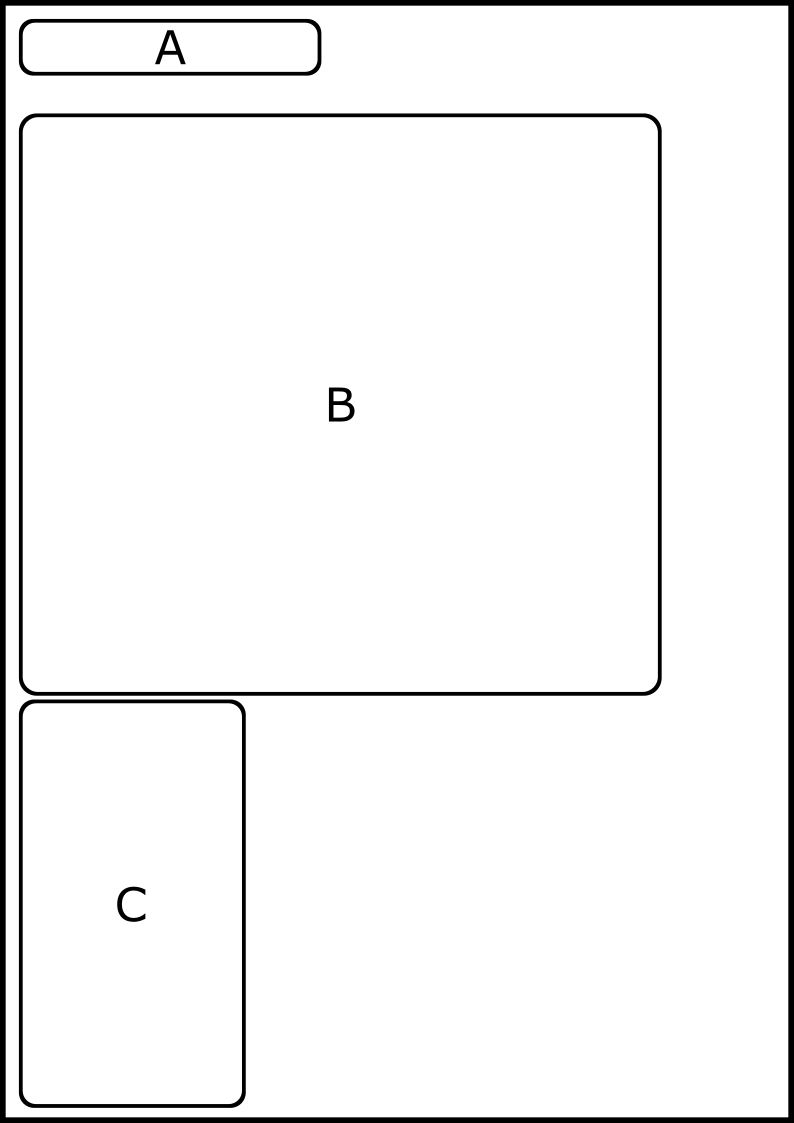
\includegraphics[width=0.4\textwidth]{images/vyzor_spravy_vylepsena}}
	%popis obrazku
	\caption[Upravené rozloženie správy]{Upravené rozdelenie správy do menšieho počtu väčších blokov}
	%id obrazku, pomocou ktoreho sa budeme na obrazok odvolavat
	\label{obr:sprava_uprava}
\end{figure}
   
\section{Predspracované dáta}
\label{predSprac}
Na účely kontroly či náš systém funguje správne sme mali v dispozícii aj niekoľko desiatok predspracovaných pacientov, čiže pacientov u ktorých sme mali ich prepúšťaciu správu a krvné výsledky a zároveň sme poznali získavané informácie. 

Problémom týchto dát však bolo, že často boli pre konkrétneho pacienta buď nekompletné alebo obsahovali informáciu ktorá sa nenachádzala ani v správe ani v krvných výsledkoch alebo boli nesprávne čo bolo spôsobené tým, že tieto dáta boli získavané iným spôsobom konkrétne tak, že poverená osoba dostala prístup do nemocničného informačného systému z ktorého následne jednotlivé dáta získavala. Konkrétne problém chýbajúcich dát boli často spôsobený tým, že v čase spracovávania pacienta daný pacient ešte nebol prepustený z nemocnice, v prípade problému dát nenachádzajúcich sa v prepúšťacej správe a krvných výsledkov išlo o prípady kedy lekár túto informáciu do prepúšťacej správy nedal a v prípade nesprávnych údajov išlo s zväčša o ľudskú chybu keďže tieto dáta boli získavané ručne.

